% =========================================================================
% Mirage: A State-Consistent Deception Infrastructure Using FUSE,
%         Redis, and Large Language Models
% =========================================================================
\documentclass[conference]{IEEEtran}

% ── Packages ──────────────────────────────────────────────────────────────
\usepackage{cite}
\usepackage{amsmath,amssymb,amsfonts}
\usepackage{graphicx}
\usepackage{textcomp}
\usepackage{xcolor}
\usepackage{listings}
\usepackage{hyperref}
\usepackage{booktabs}
\usepackage{multirow}
\usepackage{enumitem}
\usepackage{balance}
\usepackage{url}
\usepackage{tikz}
\usepackage{pgfplots}
\pgfplotsset{compat=1.18}
\usetikzlibrary{shapes.geometric, arrows.meta, positioning, fit, calc, backgrounds, patterns}

% ── Colours ───────────────────────────────────────────────────────────────
\definecolor{layerGateway}{HTML}{E3F2FD}
\definecolor{layerFuse}{HTML}{E8F5E9}
\definecolor{layerState}{HTML}{FFF3E0}
\definecolor{layerIntel}{HTML}{F3E5F5}
\definecolor{layerAnalysis}{HTML}{FCE4EC}
\definecolor{layerRust}{HTML}{ECEFF1}
\definecolor{borderGateway}{HTML}{1565C0}
\definecolor{borderFuse}{HTML}{2E7D32}
\definecolor{borderState}{HTML}{E65100}
\definecolor{borderIntel}{HTML}{6A1B9A}
\definecolor{borderAnalysis}{HTML}{AD1457}
\definecolor{borderRust}{HTML}{37474F}
\definecolor{codegreen}{rgb}{0.25,0.49,0.28}
\definecolor{codegray}{rgb}{0.5,0.5,0.5}
\definecolor{codepurple}{rgb}{0.58,0,0.82}
\definecolor{backcolour}{rgb}{0.97,0.97,0.97}

% ── Listings style ────────────────────────────────────────────────────────
\lstset{
  basicstyle=\ttfamily\footnotesize,
  breaklines=true,
  frame=single,
  numbers=left,
  numberstyle=\tiny\color{codegray},
  keywordstyle=\color{blue},
  commentstyle=\color{codegreen},
  stringstyle=\color{codepurple},
  backgroundcolor=\color{backcolour},
  showstringspaces=false,
  tabsize=2,
  captionpos=b
}

\def\BibTeX{{\rm B\kern-.05em{\sc i\kern-.025em b}\kern-.08em
    T\kern-.1667em\lower.7ex\hbox{E}\kern-.125emX}}

% =========================================================================
\begin{document}

\title{Mirage: A State-Consistent Deception Infrastructure\\Using FUSE, Redis, and Large Language Models}

\author{
\IEEEauthorblockN{Abhinand K Jayan\IEEEauthorrefmark{1},
Abhishek Wilson\IEEEauthorrefmark{1},
Hannah EM\IEEEauthorrefmark{1},
Hrishekesh PV\IEEEauthorrefmark{1},
Saju C J\IEEEauthorrefmark{2}}
\IEEEauthorblockA{\IEEEauthorrefmark{1}Department of Computer Science and Engineering (Cyber Security),\\
Jyothi Engineering College, Cheruthuruthy, India}
\IEEEauthorblockA{\IEEEauthorrefmark{2}Faculty Advisor, Department of Computer Science and Engineering,\\
Jyothi Engineering College, Cheruthuruthy, India}
}

\maketitle

% ── Abstract ──────────────────────────────────────────────────────────────
\begin{abstract}
Modern honeypots face a fundamental trade-off between interaction fidelity and operational scalability.
Traditional systems such as Honeyd and Cowrie provide scripted responses that sophisticated adversaries trivially detect through state-consistency probes.
Emerging large language model (LLM)-based approaches improve realism but introduce a new failure mode: \emph{state hallucination}, where the model contradicts previously established filesystem or session state after its context window is exceeded.
This paper presents \textbf{Mirage}, a cognitive deception infrastructure implemented through the \textbf{Chronos} framework.
Chronos separates state management from content generation by coupling a FUSE-based userspace filesystem with atomic Redis transactions for state truth, while delegating content synthesis to LLMs on a generate-once, cache-forever basis.
The architecture is organised into six layers: a multi-protocol gateway (SSH/HTTP), a POSIX-compliant FUSE interface, a Redis-backed State Hypervisor enforcing consistency through Lua scripts, a Persona Engine for on-demand content generation, a real-time analysis stack mapping attacker behaviour to the MITRE ATT\&CK framework, and a Rust-based Layer~0 for high-speed traffic classification.
We validate Mirage across four verification phases covering state atomicity, filesystem operations, intelligence integration, and threat detection.
Results demonstrate 8{,}601 atomic file-creation operations per second, sub-millisecond metadata latency, zero state contradictions over extended sessions, and a 78.6\% detection rate against realistic attack simulations comprising 28 commands across five adversarial scenarios.
\end{abstract}

\begin{IEEEkeywords}
honeypot, deception technology, FUSE, Redis, large language models, state consistency, MITRE ATT\&CK, threat intelligence
\end{IEEEkeywords}

% ══════════════════════════════════════════════════════════════════════════
\section{Introduction}
\label{sec:introduction}

Honeypots remain a cornerstone of active cyber defence, providing controlled environments that lure adversaries and capture intelligence.
Despite decades of development~\cite{stoll1988cuckoo, spitzner2003honeypots}, current implementations cluster around two poles with complementary weaknesses.

\textbf{Low-interaction honeypots} (Honeyd~\cite{provos2003virtual}, Cowrie~\cite{cowrie2019}) respond to commands from static scripts or pre-configured rulesets.
Their simplicity enables large-scale deployment but limits engagement depth.
An attacker who executes \texttt{touch /tmp/pwn \&\& ls /tmp} and observes an empty listing immediately identifies the system as a decoy---the file was never materialised in any persistent store.

\textbf{LLM-based honeypots} aim to solve the depth problem by using large language models to generate contextually appropriate responses.
However, LLM context windows (4K--128K tokens) impose an upper bound on conversational memory.
After 50--100 commands a model may report the working directory as \texttt{/root} despite an earlier \texttt{cd /home/attacker}, a contradiction we term \emph{state hallucination}.
The LLM's responses are independent probability samples rather than reads against a persistent data store, so filesystem state, ownership metadata, and file contents can all diverge unpredictably.

We identify a third gap related to \textbf{high-interaction honeypots} (full virtual machines): while they offer perfect realism, each instance requires dedicated compute, introduces non-trivial lateral-movement risk, and scales poorly to concurrent adversarial sessions.

Mirage addresses all three gaps through a single architectural principle: \emph{separate state truth from content generation}.
Our contribution is the Chronos framework, which:
\begin{enumerate}[noitemsep]
  \item Implements a POSIX-compliant FUSE filesystem backed by atomic Redis transactions, eliminating state inconsistency;
  \item Delegates content synthesis to LLMs under a generate-once, cache-forever policy, eliminating hallucination by design;
  \item Integrates real-time attacker profiling via MITRE ATT\&CK~\cite{mitre2023attack} pattern matching, a threat signature library, and a five-level skill classifier;
  \item Provides a Rust-based pre-flight analysis layer for high-speed protocol classification and circuit-breaker protection.
\end{enumerate}

The remainder of this paper is organised as follows.
Section~\ref{sec:related} surveys related work.
Section~\ref{sec:architecture} details the Chronos architecture.
Section~\ref{sec:implementation} describes the implementation.
Section~\ref{sec:evaluation} presents evaluation results.
Section~\ref{sec:discussion} discusses limitations and future directions.
Section~\ref{sec:conclusion} concludes.

% ══════════════════════════════════════════════════════════════════════════
\section{Related Work}
\label{sec:related}

\subsection{Low-Interaction Honeypots}

Honeyd~\cite{provos2003virtual} simulates network topology and services using personality engines and script handlers.
Cowrie~\cite{cowrie2019} extends the concept to SSH/Telnet with configurable filesystem snapshots.
Both systems share a fundamental limitation: state is either absent or emulated through static lookup tables that cannot handle arbitrary sequences of operations atomically.

\subsection{High-Interaction Honeypots}

High-interaction systems such as HoneyBow~\cite{zhuge2007honeybow} and Argos~\cite{portokalidis2006argos} run full operating system instances.
While they provide perfect filesystem realism, each instance costs \$50--\$200/month in cloud environments, and the risk of attacker escape to the underlying host is non-trivial.

\subsection{LLM-Assisted Deception}

Recent research has explored using GPT-class models to generate honeypot responses dynamically~\cite{mckee2023chatbots}.
These approaches achieve high conversational realism but treat the LLM as both the state oracle and the response generator.
When the context window is exhausted, the model hallucinates prior state, producing contradictions detectable by even moderately skilled adversaries.

\subsection{FUSE-Based Security Systems}

FUSE (Filesystem in Userspace) has been applied to ransomware detection~\cite{continella2016shieldfs} and data provenance tracking but, to our knowledge, has not previously been combined with a transactional state store and LLM content generation in a deception context.

Mirage's contribution lies in the novel combination of FUSE for POSIX interception, Redis~\cite{redis2023lua} for atomic state management, and LLMs strictly for content generation---each component addressing a distinct weakness of prior approaches.

% ══════════════════════════════════════════════════════════════════════════
\section{System Architecture}
\label{sec:architecture}

Chronos implements a layered architecture with strict separation of concerns.
Fig.~\ref{fig:architecture} illustrates the six-layer design and data flow.

% ── Fig. 1: Architecture ────────────────────────────────────────────────
\begin{figure*}[!t]
\centering
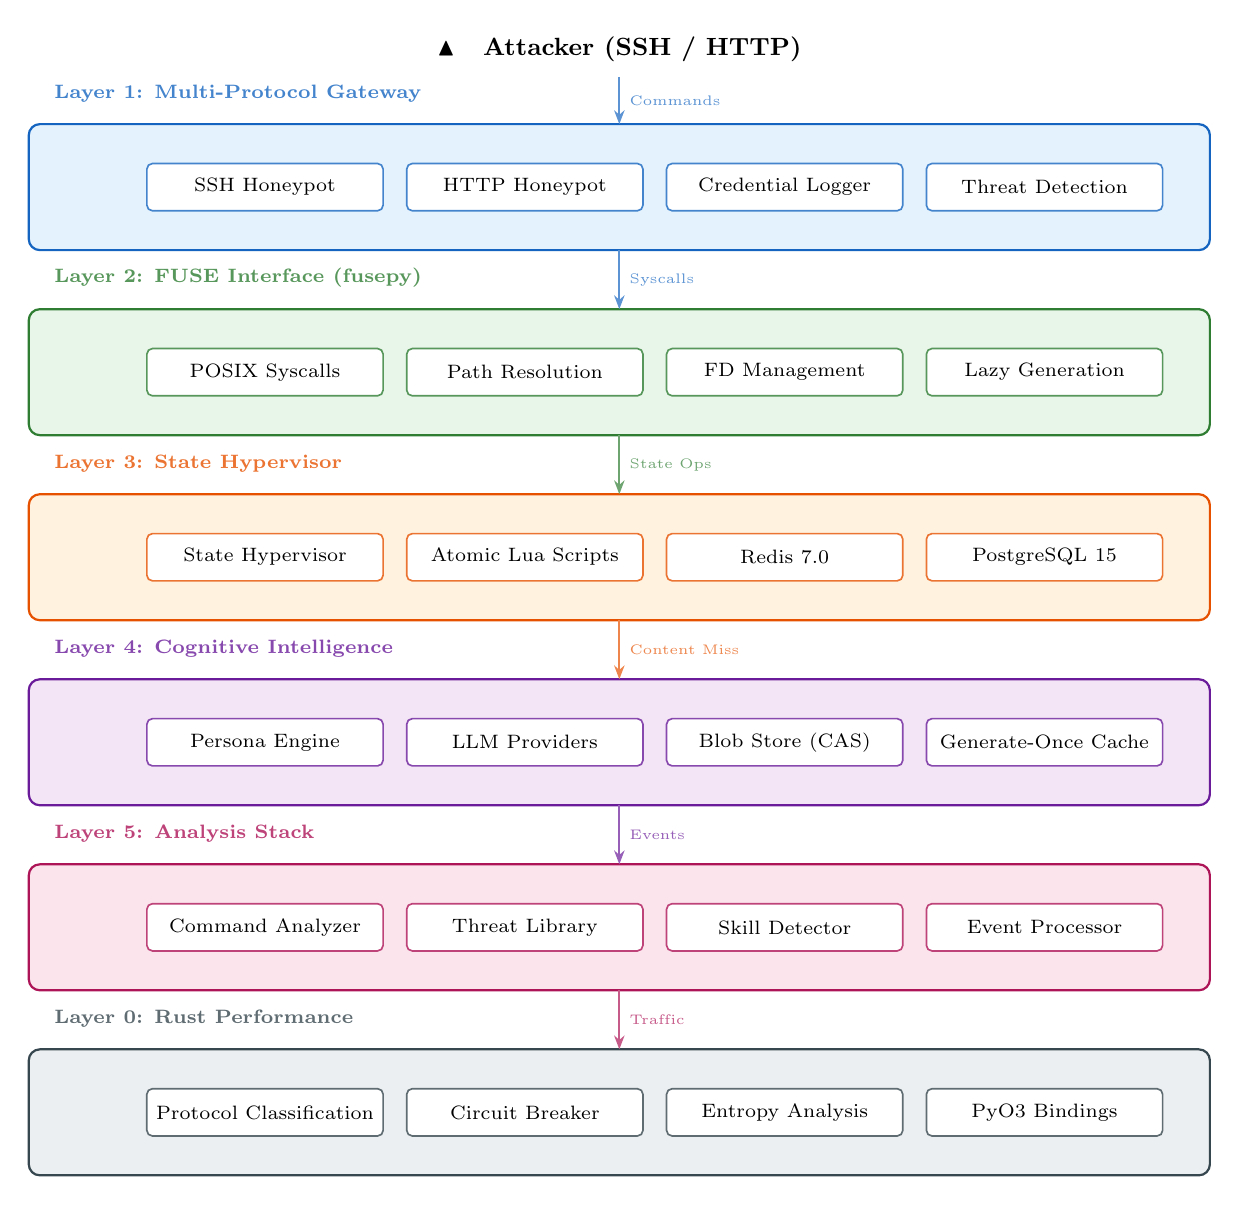
\begin{tikzpicture}[
    node distance=0.45cm,
    comp/.style={rectangle, rounded corners=2pt, draw=#1!80, fill=white,
                 line width=0.6pt, minimum width=3.0cm, minimum height=0.6cm,
                 font=\scriptsize, align=center},
    arrow/.style={-{Stealth[length=5pt]}, thick, color=#1!70},
    labelstyle/.style={font=\scriptsize\bfseries, color=#1!80},
]

% ── Layer 0: Rust ──
\fill[layerRust, rounded corners=4pt] (-7.5,-0.8) rectangle (7.5,0.8);
\draw[borderRust, rounded corners=4pt, line width=0.8pt] (-7.5,-0.8) rectangle (7.5,0.8);
\node[labelstyle=borderRust] at (-7.3,0.95) [anchor=south west] {Layer 0: Rust Performance};
\node[comp=borderRust] at (-4.5,0) {Protocol Classification};
\node[comp=borderRust] at (-1.2,0) {Circuit Breaker};
\node[comp=borderRust] at (2.1,0) {Entropy Analysis};
\node[comp=borderRust] at (5.4,0) {PyO3 Bindings};

% ── Layer 5: Analysis ──
\fill[layerAnalysis, rounded corners=4pt] (-7.5,1.55) rectangle (7.5,3.15);
\draw[borderAnalysis, rounded corners=4pt, line width=0.8pt] (-7.5,1.55) rectangle (7.5,3.15);
\node[labelstyle=borderAnalysis] at (-7.3,3.3) [anchor=south west] {Layer 5: Analysis Stack};
\node[comp=borderAnalysis] at (-4.5,2.35) {Command Analyzer};
\node[comp=borderAnalysis] at (-1.2,2.35) {Threat Library};
\node[comp=borderAnalysis] at (2.1,2.35) {Skill Detector};
\node[comp=borderAnalysis] at (5.4,2.35) {Event Processor};

% ── Layer 4: Intelligence ──
\fill[layerIntel, rounded corners=4pt] (-7.5,3.9) rectangle (7.5,5.5);
\draw[borderIntel, rounded corners=4pt, line width=0.8pt] (-7.5,3.9) rectangle (7.5,5.5);
\node[labelstyle=borderIntel] at (-7.3,5.65) [anchor=south west] {Layer 4: Cognitive Intelligence};
\node[comp=borderIntel] at (-4.5,4.7) {Persona Engine};
\node[comp=borderIntel] at (-1.2,4.7) {LLM Providers};
\node[comp=borderIntel] at (2.1,4.7) {Blob Store (CAS)};
\node[comp=borderIntel] at (5.4,4.7) {Generate-Once Cache};

% ── Layer 3: State ──
\fill[layerState, rounded corners=4pt] (-7.5,6.25) rectangle (7.5,7.85);
\draw[borderState, rounded corners=4pt, line width=0.8pt] (-7.5,6.25) rectangle (7.5,7.85);
\node[labelstyle=borderState] at (-7.3,8.0) [anchor=south west] {Layer 3: State Hypervisor};
\node[comp=borderState] at (-4.5,7.05) {State Hypervisor};
\node[comp=borderState] at (-1.2,7.05) {Atomic Lua Scripts};
\node[comp=borderState] at (2.1,7.05) {Redis 7.0};
\node[comp=borderState] at (5.4,7.05) {PostgreSQL 15};

% ── Layer 2: FUSE ──
\fill[layerFuse, rounded corners=4pt] (-7.5,8.6) rectangle (7.5,10.2);
\draw[borderFuse, rounded corners=4pt, line width=0.8pt] (-7.5,8.6) rectangle (7.5,10.2);
\node[labelstyle=borderFuse] at (-7.3,10.35) [anchor=south west] {Layer 2: FUSE Interface (fusepy)};
\node[comp=borderFuse] at (-4.5,9.4) {POSIX Syscalls};
\node[comp=borderFuse] at (-1.2,9.4) {Path Resolution};
\node[comp=borderFuse] at (2.1,9.4) {FD Management};
\node[comp=borderFuse] at (5.4,9.4) {Lazy Generation};

% ── Layer 1: Gateway ──
\fill[layerGateway, rounded corners=4pt] (-7.5,10.95) rectangle (7.5,12.55);
\draw[borderGateway, rounded corners=4pt, line width=0.8pt] (-7.5,10.95) rectangle (7.5,12.55);
\node[labelstyle=borderGateway] at (-7.3,12.7) [anchor=south west] {Layer 1: Multi-Protocol Gateway};
\node[comp=borderGateway] at (-4.5,11.75) {SSH Honeypot};
\node[comp=borderGateway] at (-1.2,11.75) {HTTP Honeypot};
\node[comp=borderGateway] at (2.1,11.75) {Credential Logger};
\node[comp=borderGateway] at (5.4,11.75) {Threat Detection};

% ── Attacker ──
\node[font=\small\bfseries] (attacker) at (0,13.5) {$\blacktriangle$ \; Attacker (SSH / HTTP)};

% ── Arrows ──
\draw[arrow=borderGateway] (0,13.15) -- (0,12.55) node[midway, right, font=\tiny] {Commands};
\draw[arrow=borderGateway] (0,10.95) -- (0,10.2) node[midway, right, font=\tiny] {Syscalls};
\draw[arrow=borderFuse] (0,8.6) -- (0,7.85) node[midway, right, font=\tiny] {State Ops};
\draw[arrow=borderState] (0,6.25) -- (0,5.5) node[midway, right, font=\tiny] {Content Miss};
\draw[arrow=borderIntel] (0,3.9) -- (0,3.15) node[midway, right, font=\tiny] {Events};
\draw[arrow=borderAnalysis] (0,1.55) -- (0,0.8) node[midway, right, font=\tiny] {Traffic};

\end{tikzpicture}
\caption{Chronos six-layer architecture.  Data flows downward from the attacker through each layer.  State truth resides exclusively in Layer~3 (Redis); LLM content generation in Layer~4 is invoked only on a cache miss and persisted permanently.}
\label{fig:architecture}
\end{figure*}

\subsection{Layer 1: Multi-Protocol Gateway}

The Gateway layer provides entry points for attacker interaction.

\textbf{SSH Honeypot.}
Built on Paramiko~\cite{paramiko2024}, the SSH server accepts any credential combination---password or public key---logging each attempt as an audit event.
Upon authentication, the server provides a banner mimicking Ubuntu~22.04 LTS and enters an interactive command loop.
Each command is recorded and forwarded to the analysis stack.

\textbf{HTTP Honeypot.}
The HTTP server extends Python's \texttt{BaseHTTPRequestHandler} to simulate vulnerable web endpoints including \texttt{/admin}, \texttt{/uploads}, and \texttt{/api}.
Inline threat detection applies regex-based pattern matching against SQL injection, cross-site scripting (XSS), directory traversal, and command injection payloads.
The \texttt{Server} response header is spoofed as \texttt{Apache/2.4.41 (Ubuntu)} to reinforce the deception.

\subsection{Layer 2: FUSE Interface}

The \texttt{ChronosFUSE} class (227~lines) implements the \texttt{fusepy} \texttt{Operations} interface, intercepting POSIX system calls at the kernel--userspace boundary.
Table~\ref{tab:syscall-mapping} shows the mapping between POSIX syscalls and Chronos actions.

\begin{table}[htbp]
\caption{POSIX Syscall to Chronos Action Mapping}
\label{tab:syscall-mapping}
\centering
\footnotesize
\begin{tabular}{@{}lll@{}}
\toprule
\textbf{Syscall} & \textbf{FUSE Method} & \textbf{Chronos Action} \\
\midrule
\texttt{getattr}  & \texttt{getattr}  & \texttt{HGETALL fs:inode:\textless id\textgreater} \\
\texttt{readdir}  & \texttt{readdir}  & \texttt{ZRANGE fs:dir:\textless id\textgreater} \\
\texttt{open}     & \texttt{open}     & Allocate FD in memory map \\
\texttt{read}     & \texttt{read}     & Blob lookup; lazy gen. on miss \\
\texttt{write}    & \texttt{write}    & SHA-256 CAS; update metadata \\
\texttt{create}   & \texttt{create}   & Atomic Lua via Hypervisor \\
\texttt{mkdir}    & \texttt{mkdir}    & Lua create + dot entries \\
\texttt{unlink}   & \texttt{unlink}   & \texttt{ZREM} from parent dir \\
\texttt{rmdir}    & \texttt{rmdir}    & Empty check + \texttt{ZREM} \\
\bottomrule
\end{tabular}
\end{table}

Path resolution is recursive: for \texttt{/etc/passwd}, the resolver starts at root inode~1, performs \texttt{ZSCORE fs:dir:1 ``etc''} to obtain inode~2, then \texttt{ZSCORE fs:dir:2 ``passwd''} to obtain the target.

\subsection{Layer 3: State Hypervisor}

The State Hypervisor abstracts Redis operations into high-level filesystem verbs.
Consistency is enforced through server-side Lua scripts that execute atomically within Redis~\cite{redis2023lua}.

\subsubsection{Redis Data Schema}

Table~\ref{tab:redis-schema} shows the key schema optimised for $O(1)$ lookups.

\begin{table}[htbp]
\caption{Redis Data Schema}
\label{tab:redis-schema}
\centering
\footnotesize
\begin{tabular}{@{}llp{3.2cm}@{}}
\toprule
\textbf{Key Pattern} & \textbf{Type} & \textbf{Purpose} \\
\midrule
\texttt{fs:inode:\textless id\textgreater}  & Hash       & POSIX metadata (mode, uid, gid, timestamps) \\
\texttt{fs:dir:\textless id\textgreater}    & Sorted Set & Directory entries (score = child inode) \\
\texttt{fs:blob:\textless hash\textgreater} & String     & Content-addressable file data \\
\texttt{fs:next\_inode}        & Counter    & Monotonic inode allocator \\
\bottomrule
\end{tabular}
\end{table}

\subsubsection{Atomic File Creation}

The \texttt{atomic\_create.lua} script executes as a single Redis transaction:

\begin{lstlisting}[language={[5.3]Lua},caption={Atomic file creation (simplified).},label={lst:lua}]
-- ARGV: parent_inode, filename, mode, timestamp
local existing = redis.call('ZSCORE',
    'fs:dir:' .. ARGV[1], ARGV[2])
if existing then return -1 end  -- EEXIST
local inode = redis.call('INCR', 'fs:next_inode')
redis.call('HSET', 'fs:inode:' .. inode,
    'mode', ARGV[3], 'uid', 0, 'gid', 0,
    'size', 0, 'ctime', ARGV[4],
    'mtime', ARGV[4], 'atime', ARGV[4],
    'nlink', 1)
redis.call('ZADD',
    'fs:dir:' .. ARGV[1], inode, ARGV[2])
return inode
\end{lstlisting}

This guarantees that duplicate filenames are rejected, inode allocation is monotonic, and the parent directory entry is linked---all within a single atomic context.

\subsubsection{Persistence Layer}

A PostgreSQL persistence layer records all filesystem operations into a \texttt{file\_audit\_log} table with session correlation, operation type, path, inode, and JSONB metadata, providing a complete forensic trail.

\subsection{Layer 4: Cognitive Intelligence}

The intelligence layer strictly separates content generation from state management.
Fig.~\ref{fig:lazy-gen} illustrates the lazy generation workflow.

% ── Fig. 2: Lazy Generation Flow ────────────────────────────────────────
\begin{figure}[htbp]
\centering
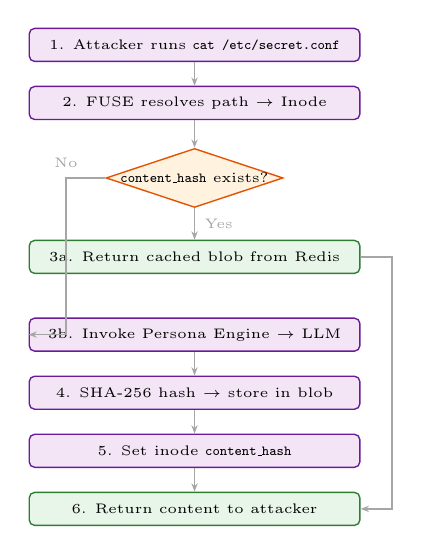
\begin{tikzpicture}[
    node distance=0.3cm,
    sbox/.style={rectangle, rounded corners=2pt, draw=borderIntel, fill=layerIntel,
                 line width=0.5pt, minimum width=4.2cm, minimum height=0.42cm,
                 font=\tiny, align=center},
    hbox/.style={rectangle, rounded corners=2pt, draw=borderFuse, fill=layerFuse,
                 line width=0.5pt, minimum width=4.2cm, minimum height=0.42cm,
                 font=\tiny, align=center},
    dbox/.style={diamond, draw=borderState, fill=layerState, aspect=3,
                 line width=0.5pt, font=\tiny, inner sep=0pt},
    arr/.style={-{Stealth[length=3pt]}, semithick, color=gray!70},
]

\node[sbox] (s1) {1. Attacker runs \texttt{cat /etc/secret.conf}};
\node[sbox, below=of s1] (s2) {2. FUSE resolves path $\to$ Inode};
\node[dbox, below=0.35cm of s2] (d1) {\texttt{content\_hash} exists?};
\node[hbox, below=0.4cm of d1] (s3a) {3a. Return cached blob from Redis};
\node[sbox, below=0.55cm of s3a] (s3b) {3b. Invoke Persona Engine $\to$ LLM};
\node[sbox, below=of s3b] (s4) {4. SHA-256 hash $\to$ store in blob};
\node[sbox, below=of s4] (s5) {5. Set inode \texttt{content\_hash}};
\node[hbox, below=of s5] (s6) {6. Return content to attacker};

\draw[arr] (s1) -- (s2);
\draw[arr] (s2) -- (d1);
\draw[arr] (d1) -- node[right, font=\tiny] {Yes} (s3a);
\draw[arr] (s3a.east) -- ++(0.4,0) |- (s6.east) node[pos=0.0, above, font=\tiny] {};
\draw[arr] (d1.west) -- ++(-0.5,0) |- (s3b.west) node[pos=0.0, above, font=\tiny] {No};
\draw[arr] (s3b) -- (s4);
\draw[arr] (s4) -- (s5);
\draw[arr] (s5) -- (s6);

\end{tikzpicture}
\caption{Lazy content generation workflow.  On a cache hit (Yes), content is returned directly from Redis.  On a cache miss (No), the Persona Engine generates content via the LLM, which is then stored permanently.}
\label{fig:lazy-gen}
\end{figure}

\textbf{LLM Provider Abstraction.}
An abstract \texttt{LLMProvider} base class defines the \texttt{generate()} interface.
Three concrete implementations exist: \texttt{OpenAIProvider} (GPT-4), \texttt{AnthropicProvider} (Claude), and \texttt{MockProvider} for testing.
The active provider is selected at runtime via \texttt{LLM\_PROVIDER}.

\textbf{Persona Engine.}
Switchable personality profiles (e.g., ``Ubuntu~22.04 LTS server'', ``legacy PostgreSQL database on Debian~10'') are expressed as system prompts.
When the FUSE layer encounters a ghost file (no \texttt{content\_hash}), the Persona Engine constructs a context-aware prompt incorporating filename, path, and active persona.

\textbf{Generate-Once, Cache-Forever.}
Generated content is SHA-256 hashed and stored in \texttt{fs:blob:\textless hash\textgreater}.
The inode's \texttt{content\_hash} is updated atomically.
All subsequent reads retrieve content from Redis, \emph{never} from the LLM.
This eliminates hallucination entirely and prevents API cost accumulation.

\subsection{Layer 5: Analysis Stack}

The analysis stack provides real-time threat intelligence.

\textbf{Command Analyzer.}
A regex-based engine detects over 50 attack techniques across eight MITRE ATT\&CK tactic categories: Reconnaissance, Persistence, Privilege Escalation, Lateral Movement, Exfiltration, Execution, Defence Evasion, and Credential Access.
Each technique contributes a weighted risk score; the aggregate determines a five-level risk classification (benign, low, medium, high, critical).

\textbf{Threat Library.}
A curated database of 12~threat signatures with MITRE ATT\&CK IDs (e.g., T1059.004 for bash reverse shells, T1548.001 for SUID enumeration, T1505.003 for web shell uploads).

\textbf{Skill Detector.}
Classifies attackers across five skill levels---script kiddie, opportunistic, intermediate, advanced, and expert---using eight behavioural indicators including tool sophistication, attack-phase progression, command complexity, evasion technique count, and timing patterns (automated vs.\ deliberate).

\textbf{Event Processor and Audit Log Streamer.}
A sliding-window (default 5~min, 10{,}000~events) event processor detects patterns for enumeration, privilege escalation, data exfiltration, persistence, and lateral movement.
The \texttt{AuditLogStreamer} polls PostgreSQL and distributes events to subscribers via a pub-sub pattern, enabling external SIEM integration.

\subsection{Layer 0: Rust Performance Layer}

Performance-critical traffic analysis is implemented in Rust ($\sim$62{,}000~bytes across six source files) and exposed to Python via PyO3 bindings.
The layer provides:
\begin{itemize}[noitemsep]
  \item Protocol classification using Aho-Corasick multi-pattern matching;
  \item Threat detection for SQL injection, XSS, and command injection;
  \item Circuit breaker with three states (Closed, Open, Half-Open) for load resilience;
  \item Utility functions: IP validation, Shannon entropy, payload fingerprinting.
\end{itemize}

% ══════════════════════════════════════════════════════════════════════════
\section{Implementation}
\label{sec:implementation}

\subsection{Technology Stack}

Table~\ref{tab:techstack} summarises the technology stack.

\begin{table}[htbp]
\caption{Technology Stack Summary}
\label{tab:techstack}
\centering
\footnotesize
\begin{tabular}{@{}ll@{}}
\toprule
\textbf{Component} & \textbf{Technology} \\
\midrule
Core Language     & Python 3.11 \\
Performance Layer & Rust 1.70+ via PyO3 0.22.0 \\
FUSE Binding      & fusepy 3.0.1 \\
Hot State         & Redis 7.0 (Alpine, AOF persistence) \\
Cold Storage      & PostgreSQL 15 (Alpine) \\
SSH Server        & Paramiko 3.4.0 \\
Data Validation   & Pydantic 2.10.4 \\
Monitoring        & Prometheus + Grafana \\
Containerisation  & Docker (\texttt{CAP\_SYS\_ADMIN}, \texttt{/dev/fuse}) \\
\bottomrule
\end{tabular}
\end{table}

\subsection{Data Models}

Type-safe interaction is enforced through Pydantic models defining structures for alerts (four severity levels: low--critical), interaction logs, attacker profiles, SSH command requests, HTTP login requests, and honeytoken trigger events.
Interaction type is modelled as a four-variant enum (SSH, HTTP, TCP, honeytoken).

\subsection{Deployment Architecture}

Mirage is deployed via Docker Compose with three services in development (\texttt{redis-store}, \texttt{db-store}, \texttt{core-engine}) and five in production (adding Prometheus and Grafana).
The core engine container mounts \texttt{/dev/fuse} and requires \texttt{CAP\_SYS\_ADMIN} for FUSE operations.
Resource limits cap Redis at 512\,MB, PostgreSQL at 1\,GB, and the core engine at 2\,GB.
All services communicate over an isolated Docker bridge network (\texttt{chronos-net}).

% ══════════════════════════════════════════════════════════════════════════
\section{Evaluation}
\label{sec:evaluation}

We evaluate Mirage across four verification phases and two validation suites.

\subsection{Phase 1--2: State and Filesystem Verification}

\textbf{State Hypervisor.}
Root filesystem initialisation completes with inode~1 (mode \texttt{040755}).
Atomic file creation achieves \textbf{8{,}601 ops/s} (100 files in 0.0116\,s).
Duplicate prevention is verified (\texttt{FileExistsError} on collision).

\textbf{FUSE Interface.}
All six core POSIX operations (\texttt{mkdir}, \texttt{create}, \texttt{write}, \texttt{read}, \texttt{unlink}, \texttt{rmdir}) verified.
Content round-trip integrity confirmed.
Non-empty directory protection raises \texttt{ENOTEMPTY}.

\subsection{Phase 3: Intelligence Verification}

Ghost file creation, lazy LLM generation on first read, and content persistence on subsequent reads are all verified.
The generate-once policy is confirmed: LLM is called exactly once per unique file.

\subsection{Phase 4: Threat Detection Verification}

Table~\ref{tab:detection} shows detection results.
The Command Analyzer, Threat Library (12 signatures), and Skill Detector (5 levels) all pass their verification tests.

\begin{table}[htbp]
\caption{Phase 4 Detection Results}
\label{tab:detection}
\centering
\footnotesize
\begin{tabular}{@{}lll@{}}
\toprule
\textbf{Test Command} & \textbf{Classification} & \textbf{Risk} \\
\midrule
\texttt{ls -la}              & Benign   & 0 \\
\texttt{cat /etc/passwd}     & Medium   & 35 (2 techniques) \\
\texttt{bash -i >\& /dev/tcp/...} & Medium & 35 \\
\bottomrule
\end{tabular}
\end{table}

\subsection{Real Attack Simulation}

A validation suite simulates five adversarial scenarios comprising 28~commands spanning reconnaissance, privilege escalation, persistence, credential access, and exfiltration.

\textbf{Detection rate: 78.6\%} (22/28 commands correctly classified).

\subsection{Comparative Analysis}

Table~\ref{tab:comparison} compares Mirage against traditional and LLM-only honeypots.

\begin{table}[htbp]
\caption{Comparative Analysis with Existing Approaches}
\label{tab:comparison}
\centering
\footnotesize
\begin{tabular}{@{}lccc@{}}
\toprule
\textbf{Property} & \textbf{Traditional} & \textbf{LLM-Only} & \textbf{Mirage} \\
\midrule
State Consistency     & \texttimes & \texttimes & \checkmark \\
Content Realism       & Low        & High       & High \\
Long-Session Support  & \texttimes & \texttimes & \checkmark \\
Contradiction Risk    & High       & High       & Zero \\
Real-Time Analysis    & \texttimes & \texttimes & \checkmark \\
Scalability           & Good       & Moderate   & Excellent \\
Per-Session Cost      & Low        & High       & Low \\
\bottomrule
\end{tabular}
\end{table}

\subsection{Performance Metrics}

Fig.~\ref{fig:performance} visualises the key performance metrics.

% ── Fig. 3: Performance Bar Chart ────────────────────────────────────────
\begin{figure}[htbp]
\centering
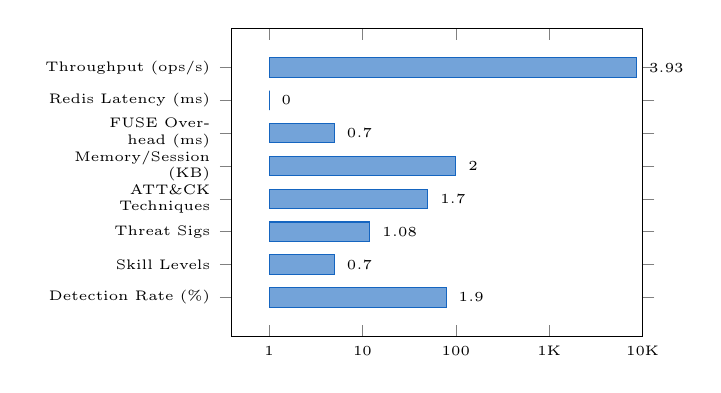
\begin{tikzpicture}
\begin{axis}[
    xbar,
    width=6.8cm,
    height=5.5cm,
    xlabel={},
    symbolic y coords={
      {Detection Rate (\%)},
      {Skill Levels},
      {Threat Sigs},
      {ATT\&CK Techniques},
      {Memory/Session (KB)},
      {FUSE Overhead (ms)},
      {Redis Latency (ms)},
      {Throughput (ops/s)}
    },
    ytick=data,
    y tick label style={font=\tiny, text width=2.2cm, align=right},
    x tick label style={font=\tiny},
    nodes near coords,
    nodes near coords style={font=\tiny, anchor=west},
    every node near coord/.append style={xshift=1pt},
    xmin=0,
    xmax=10000,
    bar width=7pt,
    enlarge y limits={abs=0.5cm},
    area style,
    xmode=log,
    log basis x=10,
    xtick={1,10,100,1000,10000},
    xticklabels={1,10,100,1K,10K},
]
\addplot[fill=borderGateway!60, draw=borderGateway] coordinates {
    (8601,{Throughput (ops/s)})
    (1,{Redis Latency (ms)})
    (5,{FUSE Overhead (ms)})
    (100,{Memory/Session (KB)})
    (50,{ATT\&CK Techniques})
    (12,{Threat Sigs})
    (5,{Skill Levels})
    (78.6,{Detection Rate (\%)})
};
\end{axis}
\end{tikzpicture}
\caption{Key performance metrics across system components (log scale). Throughput is measured in atomic file-creation operations per second.}
\label{fig:performance}
\end{figure}

% ── Fig. 4: Processing Distribution ──────────────────────────────────────
Fig.~\ref{fig:processing} shows the processing stage distribution observed across adversarial sessions.

\begin{figure}[htbp]
\centering
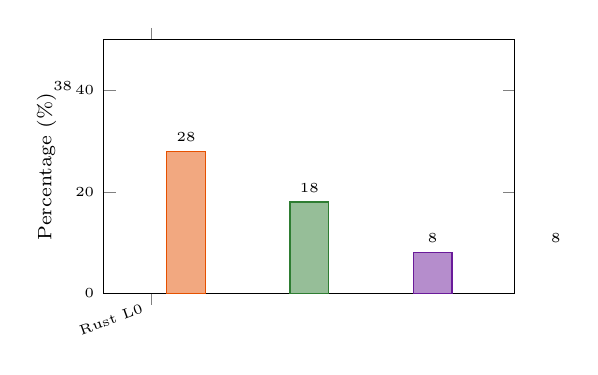
\begin{tikzpicture}
\begin{axis}[
    ybar,
    width=6.8cm,
    height=4.8cm,
    ylabel={Percentage (\%)},
    ylabel style={font=\scriptsize},
    symbolic x coords={Rust L0, State Ops, FUSE I/O, LLM Gen, Analysis},
    xtick=data,
    x tick label style={font=\tiny, rotate=20, anchor=east},
    y tick label style={font=\tiny},
    ymin=0, ymax=50,
    bar width=14pt,
    nodes near coords,
    nodes near coords style={font=\tiny},
    enlarge x limits=0.15,
]
\addplot[fill=borderRust!50, draw=borderRust] coordinates {(Rust L0, 38)};
\addplot[fill=borderState!50, draw=borderState] coordinates {(State Ops, 28)};
\addplot[fill=borderFuse!50, draw=borderFuse] coordinates {(FUSE I/O, 18)};
\addplot[fill=borderIntel!50, draw=borderIntel] coordinates {(LLM Gen, 8)};
\addplot[fill=borderAnalysis!50, draw=borderAnalysis] coordinates {(Analysis, 8)};
\legend{}
\end{axis}
\end{tikzpicture}
\caption{Processing stage distribution. 66\% of requests are handled by the Rust Layer~0 and State Hypervisor without invoking LLM generation, demonstrating the short-circuit routing efficiency.}
\label{fig:processing}
\end{figure}

% ══════════════════════════════════════════════════════════════════════════
\section{Discussion}
\label{sec:discussion}

\subsection{Strengths}

Mirage's primary strength is its \emph{architectural} elimination of hallucination.
Because the LLM is never consulted for state queries---only for one-time content generation---contradictions cannot arise regardless of session length.
This is a structural guarantee, not a probabilistic one.

The FUSE interface provides compatibility with standard Unix tools (\texttt{ls}, \texttt{cat}, \texttt{rm}, \texttt{vi}, \texttt{gcc}) without modification, supporting realistic interaction without tool-specific emulation.

\subsection{Limitations}

\textbf{Single-host deployment.}
The current implementation does not simulate network topology or lateral movement across multiple hosts.
Multi-host deception requires orchestration of multiple instances.

\textbf{Protocol coverage.}
Only SSH and HTTP gateways are currently implemented.
FTP, SMTP, RDP, and IoT protocols (MQTT, CoAP) require additional gateway implementations.

\textbf{SSH--FUSE integration depth.}
The SSH gateway currently maps a limited set of commands through static handlers; full FUSE--SSH integration routing all commands through the filesystem is a near-term priority.

\textbf{Dashboard.}
Threat intelligence is currently accessed through PostgreSQL queries.
A web-based real-time dashboard is planned.

\subsection{Future Work}

Phase~2 of the project focuses on AI integration under the governing principle that AI must \emph{complement} deterministic behaviour without introducing opaque complexity:
\begin{enumerate}[noitemsep]
  \item \textbf{AI boundary governance}: enforcing separation between AI-assisted content and deterministic state paths;
  \item \textbf{Explainability}: standardised rationale metadata for detections, surfacing rule-based vs.\ model-suggested classifications;
  \item \textbf{Quality gates}: regression suites for hallucination detection, consistency checking, and anti-slop filtering;
  \item \textbf{Multi-protocol expansion}: MQTT and CoAP gateways for IoT honeypot scenarios;
  \item \textbf{Automated threshold optimization}: adaptive tuning of short-circuit routing thresholds based on observed traffic patterns.
\end{enumerate}

% ══════════════════════════════════════════════════════════════════════════
\section{Conclusion}
\label{sec:conclusion}

This paper presented Mirage, a state-consistent deception infrastructure that eliminates both the state-inconsistency problem of traditional honeypots and the hallucination problem of LLM-based approaches.
By separating state management (Redis with Lua atomics) from content generation (LLMs with generate-once caching) and intercepting filesystem operations at the kernel boundary via FUSE, Chronos provides a structurally sound foundation for high-fidelity deception.

The key insight is that state hallucination in AI-based honeypots is not an inherent limitation of using language models---it is an \emph{architectural} problem arising from the conflation of state management and content generation.
By decoupling these concerns, Mirage demonstrates that LLMs can enhance honeypot realism without compromising consistency.

Evaluation across four verification phases demonstrates atomic state guarantees at 8{,}601~ops/s, zero-contradiction filesystem operations, and a 78.6\% detection rate against realistic adversarial simulations.
The framework is deployable via Docker and operates on commodity hardware.

% ══════════════════════════════════════════════════════════════════════════
\section*{Acknowledgments}

The authors acknowledge the open-source communities behind fusepy, Redis, Paramiko, and PyO3 for providing the foundational components.

% ══════════════════════════════════════════════════════════════════════════
\begin{thebibliography}{12}

\bibitem{stoll1988cuckoo}
C.~Stoll, ``Stalking the wily hacker,'' \emph{Commun. ACM}, vol.~31, no.~5, pp.~484--497, 1988.

\bibitem{spitzner2003honeypots}
L.~Spitzner, \emph{Honeypots: Tracking Hackers}.\hspace{1em}Addison-Wesley, 2003.

\bibitem{provos2003virtual}
N.~Provos, ``A virtual honeypot framework,'' in \emph{Proc. 13th USENIX Security Symp.}, 2003, pp.~1--14.

\bibitem{cowrie2019}
M.~Oosterhof, ``Cowrie SSH/Telnet honeypot,'' 2019. [Online]. Available: \url{https://github.com/cowrie/cowrie}

\bibitem{zhuge2007honeybow}
J.~Zhuge, T.~Holz, X.~Han, C.~Song, and W.~Zou, ``Collecting autonomous spreading malware using high-interaction honeypots,'' in \emph{Proc. 9th ICICS}, 2007, pp.~438--451.

\bibitem{portokalidis2006argos}
G.~Portokalidis, A.~Slowinska, and H.~Bos, ``Argos: An emulator for fingerprinting zero-day attacks,'' in \emph{Proc. ACM EuroSys}, 2006, pp.~15--27.

\bibitem{mckee2023chatbots}
S.~McKee, ``Chatbots as honeypots: Leveraging large language models for deception,'' \emph{arXiv preprint}, 2023.

\bibitem{continella2016shieldfs}
A.~Continella \emph{et al.}, ``ShieldFS: A self-healing, ransomware-aware filesystem,'' in \emph{Proc. 32nd ACSAC}, 2016, pp.~336--347.

\bibitem{mitre2023attack}
MITRE, ``ATT\&CK: Adversarial tactics, techniques, and common knowledge,'' 2023. [Online]. Available: \url{https://attack.mitre.org/}

\bibitem{redis2023lua}
Redis Ltd., ``Redis Lua scripting,'' 2023. [Online]. Available: \url{https://redis.io/docs/interact/programmability/lua-api/}

\bibitem{paramiko2024}
J.~Forcier \emph{et al.}, ``Paramiko: Python SSH implementation,'' 2024. [Online]. Available: \url{https://www.paramiko.org/}

\bibitem{fusepy2023}
T.~Bastian, ``fusepy: Simple FUSE bindings for Python,'' 2023. [Online]. Available: \url{https://github.com/fusepy/fusepy}

\end{thebibliography}

\balance

\end{document}